\section{Design}

FlashMatrix is a matrix-oriented programming framework for general data analysis.
This work mainly focuses on dense matrices and scales
dense matrix operations beyond memory capacity by utilizing fast I/O devices,
such as solid-state drives (SSDs), in a non-uniform memory architecture (NUMA).
FlashMatrix uses R as its main programming interface and executes R code
automatically in parallel and out of core.

Figure \ref{fig:arch} shows the architecture of FlashMatrix. The main programming
interface comprises a small number of generalized matrix operators (GenOps).
As such, FlashMatrix only focuses on optimizations on these GenOps
to greatly simplify the implementation and improve the expressiveness of
the framework. The optimizer in FlashMatrix aggressively merges operators to
reduce CPU cache misses and I/O accesses and achieve better parallelization.
FlashMatrix stores large matrices on SSDs through SAFS \cite{safs},
a user-space filesystem for a large SSD array, to fully utilize high I/O
throughput of the SSDs and deploys a set of I/O optimizations to improve
its sequential I/O throughput \cite{SEM_SpMM}.

\begin{figure}
\centering
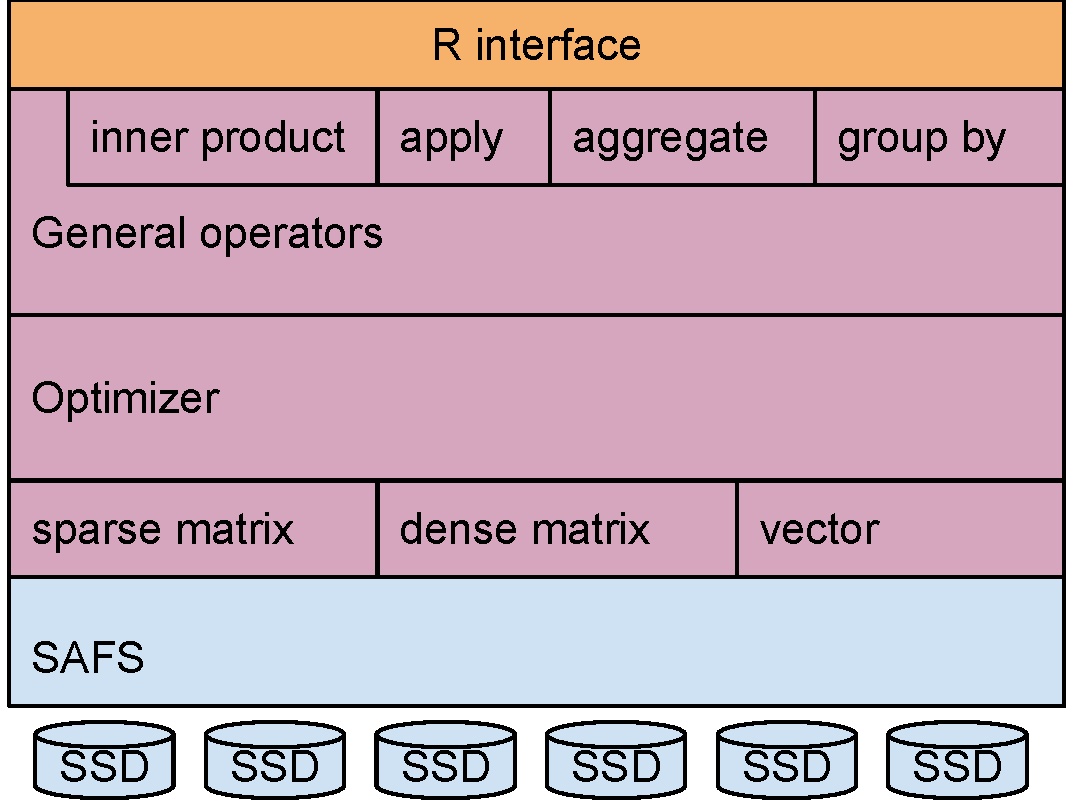
\includegraphics[scale=0.3]{./architecture.pdf}
\caption{The architecture of FlashMatrix.}
\label{fig:arch}
\end{figure}

FlashMatrix provides an matrix-oriented functional programming interface.
It exposes GenOps in its R interface and reimplements many functions
in the R \textit{base} package with the GenOps. Every function operates on
one or more matrices and outputs a new matrix. As such, the matrices in
FlashMatrix are immutable. The functions provided by the R interface are
categorized into seven classes:
\begin{itemize}
	\item The generalized matrix operators (GenOps).
	\item The construction functions that create vectors and matrices of
		the specified size and fill them with specified data (e.g., sequence
		number or random number).
	\item The conversion functions that convert between FlashMatrix matrices and
		R matrices to enable interaction between FlashMatrix and the R framework.
	\item The transformation functions that change the shape of a matrix.
		The commonly used functions include matrix transpose, matrix combination
		such as \textit{rbind} and \textit{cbind} and submatrix extraction.
	\item Element-wise operations such as matrix addition and subtraction.
	\item Aggregation operations such as summation.
	\item BLAS matrix multiplication.
\end{itemize}

%\subsection{SAFS}

%SAFS \cite{safs} is a user-space filesystem for a high-speed SSD array in
%a NUMA machine. It is implemented as
%a library and runs in the address space of its application. It is deployed
%on top of the Linux native filesystem. SAFS was originally designed for
%optimizing small I/O accesses. However, FlashMatrix accesses data in matrices
%sequentially and
%generates much fewer but much larger I/O. Therefore, we provide additional
%optimizations to maximize sequential I/O throughput from a large SSD array.

%The first optimization is to enable polling for I/O to reduce thread context
%switches. On a high-speed SSD array, the latency caused by a thread context
%switch becomes noticeable under a sequential I/O workload and it becomes
%critical to avoid thread
%context switch to gain I/O performance. If the computation in application
%threads does not saturate CPU, SAFS will put the application threads into
%sleep while they are waiting for I/O. This results in many thread context
%switches and underutilization of both CPU and SSDs. To saturate I/O,
%an application thread issues asynchronous I/O to SAFS and poll for I/O
%completion after completing all computation available to it. Polling avoids
%a thread from being switched out during I/O access and effectively maximizes
%I/O throughput of a high-speed SSD array.

%To better support access to many files simultaneously, SAFS stripes data in
%a file across SSDs with a different striping order for each file. Due to
%the sequential I/O workload, FlashMatrix stripes data across SSDs with a large
%block size, on the order of megabytes, to increase I/O throughput and reduce
%write amplification on SSDs \cite{Tang15}. Such a large block size may cause
%storage skew for small files on a large SSD array if every file stripes data
%in the same order. Using the same striping order also causes skew in I/O access.
%Therefore, SAFS generates a random striping order for each file to evenly
%distribute I/O among SSDs. SAFS stores the striping order with a file for
%future data retrieval.

%When accessing a file sequentially from SSDs, we maintain a set of memory buffers
%for I/O access to reduce the overhead of memory allocation.
%We use large I/O to increase I/O throughput. As such, we need to allocate
%a large memory buffer for I/O access.
%The operating system usually allocates a large memory buffer with \textit{mmap()}
%and populates the buffer with physical pages when it is used. It is
%computationally expensive to populate
%large memory buffers frequently. When accessing high-throughput I/O devices,
%such overhead can cause substantial performance loss. Therefore, we keep a set
%of memory buffers allocated previously and reuse them for new I/O requests.

\subsection{Dense matrices}
Dense matrices are the main data types in FlashMatrix. A vector is stored
as a one-column dense matrix. In FlashMatrix, a dense matrix can be physically
stored in memory or on SSDs or represented virtually by a sequence of computation.

%A matrix has two identifiers: the \textit{matrix identifier} that indicates
%the matrix itself and the \textit{matrix data identifier} that indicates
%the data in the matrix. When a matrix is cloned or transposed, the new matrix
%has a different \textit{matrix identifier} but shares the same
%\textit{matrix data identifier} with the original matrix.

\subsubsection{Tall-and-skinny matrices} \label{sec:tas_mat}

FlashMatrix optimizes for tall-and-skinny (TAS) dense matrices due to their
frequent occurrence in many data analysis tasks.
In data analysis and machine learning, many data matrices contain a large
number of samples with a relatively few attributes, so the shape
of the data matrices is usually tall and skinny. If a data matrix has many
attributes, the first step is usually dimension reduction \cite{} and
the operation results in a tall-and-skinny matrix. FlashMatrix specifically
optimizes for TAS dense matrices with tens of columns or fewer.
This section describes optimizations on TAS matrices and the same optimizations
is applied to short-and-wide matrices.

FlashMatrix supports row-major and column-major matrix layout (Figure
\ref{fig:tas_mat}). As such,
we avoid data copy for matrix operations such as matrix transpose.
Furthermore, each GenOp has its own preferred matrix layout. FlashMatrix
optimizes matrix operations for both data layouts. The layout of an output
matrix is generally determined by a GenOp. Columns in a column-major TAS matrix
are not stored contiguously.

\begin{figure}
	\centering
	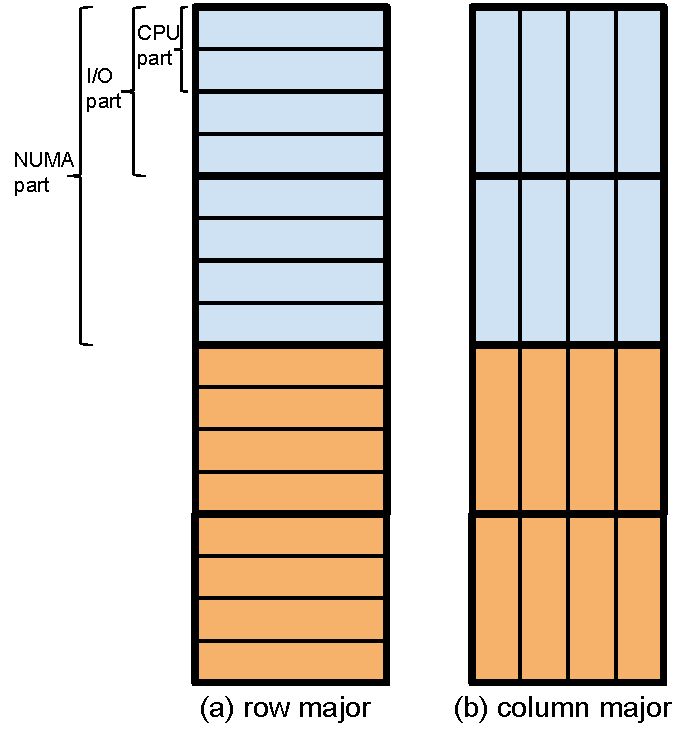
\includegraphics[scale=0.5]{./dense_matrix.pdf}
	\caption{The format of a tall-and-skinny dense matrix.}
	\label{fig:tas_mat}
\end{figure}

FlashMatrix uses two-level horizontal partitioning on TAS matrices for efficient
data access to SSDs and main memory (Figure \ref{fig:tas_mat}). Both in-memory
and external-memory TAS matrices are first partitioned horizontally into
I/O-level partitions. All elements in an I/O-level partition are stored
contiguously regardless of the data layout in the matrix. For an in-memory matrix,
the partition size determines the size of contiguous memory required in memory
allocation (see Section \ref{sec:mem}). For an external-memory matrix, each I/O
access reads the entire I/O-level partition. The partition size determines an I/O
size, usually in the order of megabytes. The number of rows in an I/O-level
partition is always $2^i$. This produces column-major TAS matrices whose data
are well aligned in memory to help CPU vectorization.
We further split an I/O-level partition
horizontally into CPU-level partitions for computation. We use a small
CPU-level partition (in the order of kilobytes) so that it fits in CPU L1/L2
cache to reduce CPU cache misses when evaluating a sequence of matrix
operations (Section \ref{sec:lazy_eval}). FlashMatrix determines the number
of rows in a CPU-level partition based on the number of columns in a matrix.

%\begin{itemize}
%\item NUMA-level partitioning: When a TAS
%matrix is stored in memory, it is partitioned across NUMA nodes to achieve
%data locality and fully utilize memory bandwidth. NUMA-level partitioning
%maps partitions of different vectors/matrices involved in computation
%to the same NUMA node to reduce inter-processor communication. As such,
%the partition size (the number of rows in a partition) is a global parameter
%and is not affected by the number of columns in a matrix.
%\end{itemize}

\subsubsection{Virtual matrices} \label{virt_mat}
In many cases, we do not need to store the data of a matrix physically. Instead,
we compute and generate its data on the fly. \textit{virtual matrices} store
computation and potentially the reference
to some other matrices required by the computation. A simple example is a matrix
with all elements having the same value. For such a matrix, we only need to store
a single value and construct its matrix partitions during computation.

\textit{Virtual matrices} are essential for lazy evaluation (Section
\ref{sec:lazy_eval}). All GenOps may output \textit{virtual matrices} that
represent the computation result and only store the computation of the GenOps
and the references to the input matrices of the GenOps. This strategy is
essential for both in-memory and external-memory optimizations to improve
performance. It significantly reduces data access to memory and SSDs and
memory allocation overhead.

%\subsubsection{Cached matrix}
%Memory cache is necessary for external-memory matrices on a machine with
%substantial memory.
%Even though SSDs have significantly improved I/O performance, they are still
%an order of magnitude slower than DRAM. Unfortunately, we cannot rely on
%the page cache in SAFS \cite{sa-cache} to buffer some portion of a dense matrix
%because streaming a matrix to memory always evicts existing data in the page
%cache and generates zero cache hits. Therefore, we explicitly cache some portion
%of a dense matrix.

%We store a matrix cache as an in-memory dense matrix.
%To effectively cache data in a dense matrix, we store a tall matrix in
%column-major and cache the first few columns; we store a wide matrix in row-major
%and cache the first few rows. As such, when computation requests an I/O-level
%partition of a matrix, we only need to issue a single I/O request to read
%the remaining columns or rows to reconstruct the I/O-level partition.

%We use a write-through policy for the matrix cache. As such, even when part of
%a dense matrix is cached, we keep a complete copy of the dense matrix on SSDs.
%The benefit of a write-through policy is to overlap computation and I/O when
%a dense matrix is created and avoid I/O latency when removing the cache.

\subsubsection{A group of dense matrices} \label{sec:mat_group}
FlashMatrix represents a tall matrix with many columns with a group of
tall-and-skinny matrices and a wide matrix with a group of short-and-wide
matrices. We construct a special \textit{virtual matrix} to represent
a group of dense matrices. To take advantage of the optimizations on matrix
operations on TAS matrices, we decompose a matrix operation on a group of
matrices into operations on individual matrices in the group (Section
\ref{sec:group_op}).
Coupled with the two-level partitioning on TAS matrices, this strategy enables
2D-partitioning on a dense matrix and each partition fits in main memory
or CPU cache.

%\begin{figure}
%	\centering
%	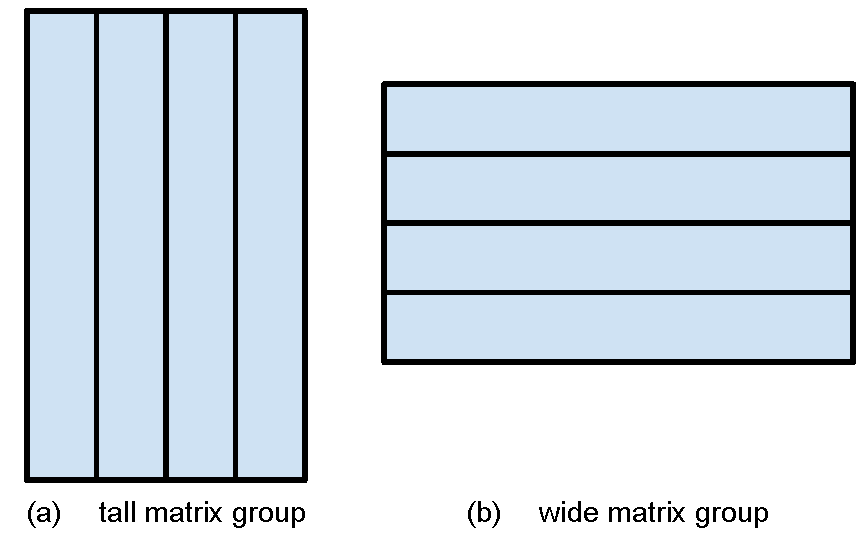
\includegraphics[scale=0.5]{./matrix_group.pdf}
%	\caption{A group of matrices to form a tall matrix with many columns (a)
%	and a wide matrix with many rows (b).}
%	\label{fig:mat_group}
%\end{figure}

%A group of matrices should be stored in a single SAFS file to reduce the number
%of SAFS files.

%append an element to a vector can be implemented as physically appending the element
%to the vector. The result vector becomes the new vector, and the original vector
%becomes the sub-vector of the new vector.

\subsection{Generalized computation operations} \label{sec:genop}
To improve generality and simplify the implementation, FlashMatrix provides
only four generalized operators (GenOps) on matrices: \textit{inner product},
\textit{apply}, \textit{aggregation} and \textit{groupby}. Each of the operators
represents a data access pattern and accepts some functions as additional
arguments that define computation
on individual elements in matrices (Section \ref{sec:vudf}).

\textit{Inner product} is a generalized matrix multiplication. It replaces
multiplication and addition in matrix multiplication with two functions.
We define many operations
with inner product. For example, we use inner product to compute various
pair-wise distances between samples such as Euclidean distance and
Hamming distance. For dense matrices, we mainly focus on
optimizing two cases: inner product of a wide matrix and a tall matrix (denoted
with \textit{inner\_prod\_wide}) and inner product of a tall matrix and a small
matrix (denoted with \textit{inner\_prod\_tall}). It is impractical to
materialize inner product of a large tall matrix and a large wide matrix owing
to space complexity. This holds for all matrix algebra frameworks.
%Common
%practice transforms computation that requires this form of inner product to
%the other two forms to reduce space complexity \cite{}.
Even though we can implement matrix multiplication with inner product,
FlashMatrix relies on BLAS to implement matrix multiplication for
floating-point matrices to achieve speed and precision required by
many numeric libraries, such as eigensolvers \cite{anasazi, FlashEigen}.

\textit{Apply} is a generalized form of element-wise operations and has
multiple variants. The simplest variant (denoted with \textit{sapply}) is
an element-wise unary operation. We use it to implement many unary
operations such as negation, square root or element type casting
on a matrix. The second variant (denoted with \textit{mapply}) is an
element-wise binary operation. We use it to implement many binary
matrix operations such as matrix addition and subtraction. The third
(denoted with \textit{mapply\_row}) and the fourth variants (denoted with
\textit{mapply\_col}) perform element-wise
binary operation on the input vector with every row or column of the input
matrix and output a matrix with the same shape as the input matrix.
%Although
%\textit{mapply\_row} and \textit{mapply\_col} can also be implemented by
%replicating the input vector to create a matrix and applying \textit{mapply}
%on the input matrix and the created matrix, \textit{mapply\_row} and
%\textit{mapply\_col} avoid CPU cache polution to improve performance.

\textit{Aggregation} takes multiple elements and outputs a single element.
It has three variants on a matrix. The first variant (denoted with \textit{agg})
aggregates over all elements on a matrix, e.g., matrix summation. The second
(denoted with
\textit{agg\_row}) and the third variants (denoted with \textit{agg\_col})
compute aggregation over each individual row or column. \textit{rowSums}
and \textit{colSums} in R are examples.

\textit{Groupby} on a matrix groups rows (\textit{groupby\_row}) or columns
(\textit{groupby\_col}) of a matrix based on a vector of categorical values
and perform aggregation on the rows or
columns associated with the same categorical value. Matrix \textit{groupby}
is used in classification and clustering algorithms that compute
aggregation on the data points in a class or in a cluster.

\subsection{Vectorized user-defined function} \label{sec:vudf}
GenOps take functions that define computation on individual elements,
which potentially results in significant function call overhead. All of
the GenOps take vectorized user-defined functions (VUDFs) that operate on
a vector of elements instead of an individual element. By transforming
the operations on individual elements to the ones on a vector, we amortize
the overhead of function calls significantly.
%GenOps accept the pointers to VUDFs at runtime to support
%dynamic programming languages such as R.

We balance the amortization of function call overhead and CPU cache misses.
To reduce latency of accessing data in VUDFs,
the input data has to be small enough to fit in the CPU L1 cache. On the
other hand, passing a longer vector to a VUDF amortizes the overhead of
function calls more aggressively. We use 128 as the maximum length of
the input vector of a VUDF. %Futher increasing the length does not have
%noticeable performance improvement.

We have three types of VUDFs to support the GenOps in FlashMatrix. Each VUDF
type may have multiple forms to allow GenOps to transform operations to
increase the length of an input vector to a VUDF and increase amortization
of function call overhead.
\begin{itemize}
	\item A \textit{unary} VUDF (denoted with \textit{uVUDF}) takes a vector
		as input and outputs a vector of the same length.
	\item A \textit{binary} VUDF has three forms: the first form (denoted with
		\textit{bVUDF1}) takes two vectors of the same length and outputs
		a vector of the same length as the input vectors; the second form (denoted
		with \textit{bVUDF2}) takes a vector as the left argument and a scalar
		as the right argument and outputs a vector with the same length as
		the input vector; the third form (denoted with bVUDF3) takes a scalar
		as the left argument and a vector as the right argument and outputs
		a vector. The second and third forms support non-commutative binary
		operations such as division and subtraction.
	\item An \textit{aggregation} VUDF consists of two functions:
		\textit{aggregate} and \textit{combine}. Both functions may have two
		forms: the first one (denoted with \textit{aVUDF1}) takes a vector and
		outputs a scalar; the second one (denoted with \textit{aVUDF2}) takes
		two vectors of the same length and outputs a vector. For many
		aggregation VUDFs such as summation, \textit{aggregate} and
		\textit{combine} are the same and have both \textit{aVUDF1} and
		\textit{aVUDF2} forms. For some aggregation such as \textit{count},
		\textit{aggregate} and \textit{combine} are different.
\end{itemize}

Figure \ref{fig:DAG} shows an example of using GenOps and VUDFs to compute
standard deviation on a matrix with missing values. Standard deviation is
computed with the following
formula: $\sigma = \sqrt{E[X^2] - (E[X])^2}$, where $X$ is the input matrix and
$E[X]$ is the mean of the matrix $X$. In the presence of missing values, we
need to exclude the missing values from the matrix. The first step is to apply
$sapply$ with the unary VUDF $sq$ to compute $X^2$ and apply $sapply$ with
the unary VUDF $isna$ to test which elements are missing values. The second
step is to apply $mapply$ with the binary VUDF $ifelse0$ on $X$ and $isna.X$
to replace missing
values in $X$ with 0 and on $X^2$ and $isna.X$ to replace missing values in
$X^2$ with 0. The third step is to apply $agg$ with $+$ to compute summation
of $X$, $X^2$ and $isna.X$. Eventually, we compute the mean of $X$ and
$X^2$ and the standard deviation, excluding missing values.

FlashMatrix provides many commonly used VUDFs. These VUDFs wrap
basic operations built in many programming languages and libraries. For example,
FlashMatrix provides arithmetic operations such as \textit{addition} and
\textit{subtraction}, relational operations such as \textit{equal to} and
\textit{less than}, logical operations such as \textit{logical AND} and
\textit{logical OR}, as well as commonly used math functions such as computing
absolute values and square root. FlashMatrix also provides a set of VUDFs to
cast primitive element types.

For each basic operation in a VUDF, FlashMatrix provides multiple VUDF
implementations to support different element types. To reduce the number
of binary VUDF implementations, FlashMatrix only provides the ones that take
two input arguments of the same type. If a GenOp gets two matrices with different
element types, it first casts the element type of one matrix to match
the other. Type casting follows the usual arithmetic conversions \cite{}
commonly seen in many programming languages. Type casting operations are
implemented with \textit{sapply} and are performed lazily.

FlashMatrix allows programmers to extend the framework by registering new VUDFs.
Like built-in VUDFs, a new VUDF needs to provide multiple
implementations to support different element types; based on the type of
the VUDF, it may need to provide different forms as described above.
FlashMatrix currently requires a VUDF to be implemented with C/C++.

We use CPU vector instructions such as AVX \cite{avx} to accelerate
the computation in a VUDF. The current implementation of FlashMatrix heavily
relies on auto-vectorization of a compiler, such as GCC, to vectorize
computaion. FlashMatrix provides hints and
transforms code to help auto-vectorization. For example, a VUDF in FlashMatrix
frequently operates on vectors with data well aligned in memory and of
the length defined at compile time, so we inform the compiler of the data alignment
and the vector length. Some compilers do not automatically vectorize
aggregation operations well. We manually create a small vector of reduction
variables, flatten the loop and transform the original aggregation operation
into aggregation onto the vector of reduction variables.

\subsection{Lazy evaluation} \label{sec:lazy_eval}
FlashMatrix evaluates matrix operations lazily. Evaluating individual
matrix operations results in significant data movement between CPU and SSDs
and frequent memory allocation in in-memory execution.
Lazy evaluation enables matrix operation fusion to minimize data movement,
reduce memory allocation overhead and improve parallelization \cite{Ching12}.

\begin{figure}
	\centering
	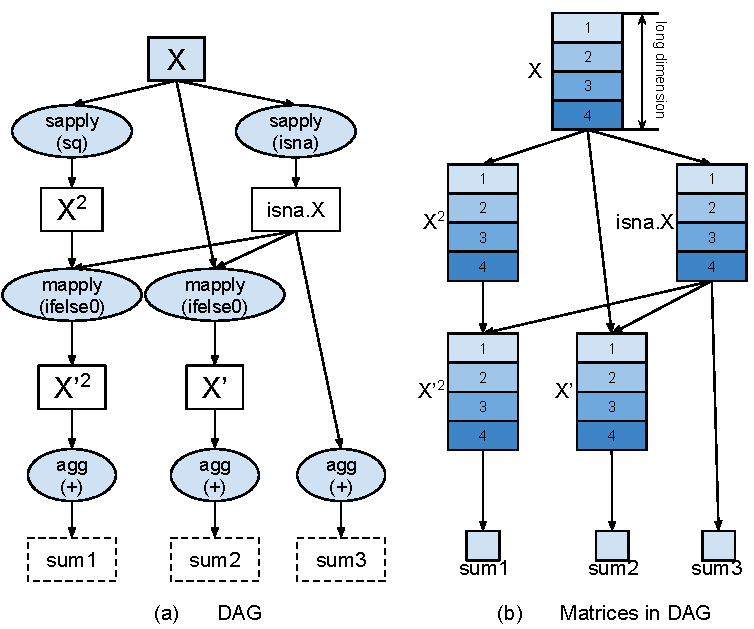
\includegraphics[scale=0.7]{./sd.pdf}
	\caption{A directed acyclic graph of computing standard deviation on
	a matrix with missing values.}
	\label{fig:DAG}
\end{figure}

FlashMatrix constructs a directed acyclic graph (DAG) to represent
computation formed by a sequence of matrix operations evaluated lazily
(Figure \ref{fig:DAG} (a)). A lazily evaluated GenOp outputs a \textit{virtual matrix}
to capture the matrix computation and the input matrices. As such, a computation
DAG is formed with a set of \textit{virtual matrix} nodes (shown as rectangles)
and computation nodes (shown as ellipses). We refer to the input matrices of
a computation node as the parent matrices and the output matrix as the child matrix.
The computation nodes may contain some immutable computation state such as
scalar variables and small matrices involved in the matrix computation.
A matrix node can be used by multiple computation nodes as
an input matrix. Although the \textit{virtual matrices} do not need to have
the same shape, FlashMatrix requires all \textit{virtual matrices} in the DAG
has the same \textit{long dimension} size (Figure \ref{fig:DAG} (b)) to
simplify evaluation and data flow of a DAG (a \textit{long dimension}
refers to the matrix dimension with the larger size).

FlashMatrix allows lazy evaluation on all GenOps. There are two types of GenOps
in a DAG: the ones such as \textit{sapply} and \textit{mapply} that output
matrices with the same \textit{long dimension} size as the input matrices
and the ones such as \textit{agg} and \textit{groupby} that output matrices
with different \textit{long dimension} sizes. The output matrices of the first
type of GenOps can be easily connected to other nodes in a DAG. Any computation
that uses the output matrices of the second type of GenOps as input cannot be
connected to the same DAG and we refer to these output matrices as
\textit{sink matrices}.

To enable lazy evaluation, all matrices in FlashMatrix are immutable and every
matrix operation generates a new matrix. As such, \textit{virtual matrices}
generate the same result every time they are materialized. FlashMatrix
garbage collects a matrix when there are no references to it.

\subsection{Matrix materialization} \label{sec:materialize}
Lazy evaluation postpones computation in matrix operations, but we eventually
have to perform actual computation and materialize some \textit{virtual matrices}.

FlashMatrix allows to materialize any \textit{virtual matrix} in a DAG and
can materialize multiple \textit{virtual matrices} together. Typically, we
materializes only \textit{sink matrices} in a DAG. In the example shown in
Figure \ref{fig:DAG}, we materialize the three \textit{sink matrices} together
to reduce data movement in memory hierarchy. Many iterative algorithms need
to materialize some non-\textit{sink matrices} in a DAG to avoid redundant
computation and I/O because the non-\textit{sink matrices} are used
in the next iteration. FlashMatrix allows users to set a flag on the
non-\textit{sink matrices} to inform FlashMatrix to save materialized data
of these matrices to memory or SSDs during computation.

We partition matrices on a DAG in the \textit{long dimension} for materialization
and parallelization (Figure \ref{fig:DAG} (b)). All \textit{virtual matrices}
except \textit{sink matrices} on a DAG have the same \textit{long dimension}
size. To simplify materialization, they all share the same partition size in
the \textit{long dimension}.
As such, a partition $i$ of a \textit{virtual matrix} only requires data from
partitions $i$ of the parent matrices and partitions in a matrix are
evaluated independently. %By default, FlashMatrix discards data in a partition
%immediately once the data is used by all children matrices.
%Owing to the storage scheme for
%in-memory matrices, the data of all in-memory matrices in a partition are stored
%on the same NUMA node to minimize remote memory access.
A \textit{sink matrix} is an output of some form of aggregation on its parent
matrix. When materializing a \textit{sink matrix}, each thread computes partial
aggregation results on the partitions of the parent matrix assigned to the thread.
In the end of computation, FlashMatrix merges the partial aggregation results to
construct the \textit{sink matrix}.

%\textit{sink matrices} are usually small and are materialized in memory.
%For example, \textit{agg\_row} on a wide matrix and
%\textit{agg\_col} on a tall matrix outputs a vector. The maximal length of
%the vector is $\sqrt{N}$, where $N$ is the number of elements
%in the input matrix. As such, we can always keep it in memory. For most of machine
%learning and data analysis tasks, the output matrix of the inner product of
%a wide matrix with a tall matrix is usually small and is by default kept
%in memory because the long dimension of these matrices is usually much larger
%than the short dimension in these tasks.

FlashMatrix takes advantage of the two-level
partitioning on dense matrices to reduce data movement between SSDs and CPU.
It assigns I/O-level partitions (Section \ref{sec:tas_mat}) to a thread as
computation tasks for parallelization. We choose a relatively small partition
size to balance the overhead of accessing a partition, parallelization skew
and memory consumption. A thread further splits an I/O-level partition into
CPU-level partitions at run time and materializes one CPU-level partition at
a time. When a CPU-level partition is materialized, it is passed to the
subsequent operation in the DAG. A CPU-level partition is sufficiently small
to fit in the CPU cache so that the partition still resides in CPU cache when
it is consumed by the subsequent operation. %In a DAG, a matrix may be
%required by multiple GenOps. As such, each matrix always buffers one materialized
%CPU-level partition in each thread to avoid redundant computation.
%\dz{We need to identify transpose of a matrix.}

%FlashMatrix uses a global task scheduler to assign tasks to threads dynamically
%for load balancing and I/O merging. However, SSDs require large
%writes to achieve sustainable write throughout and reduce write amplification
%\cite{}. As such, FlashMatrix delays writing the materialized partitions to
%SSDs and merge multiple materialized partitions into a single write because
%the global task scheduler assigns consecutive partitions to threads.

%To keep data in CPU cache as long as possible, we reuse the memory buffers
%to reduce the number of memory buffers used in the computation and avoid CPU
%cache polution.

\subsection{Memory management} \label{sec:mem}
FlashMatrix manages large memory allocation to reduce memory allocation overhead.
In-memory matrix creation and I/O access to matrices on SSDs require large memory
allocation. The functional programming interface of FlashMatrix leads to more
frequent memory allocation because each matrix operation generates a new matrix. 
Large memory allocation is expensive in Linux because Linux uses \textit{mmap}
to allocate large memory and relies on page fault to populate the memory.
Frequent page faults prevent computation from fully utilizing CPUs in a large
parallel machine and causes significant performance degradation.

\begin{figure}
	\centering
	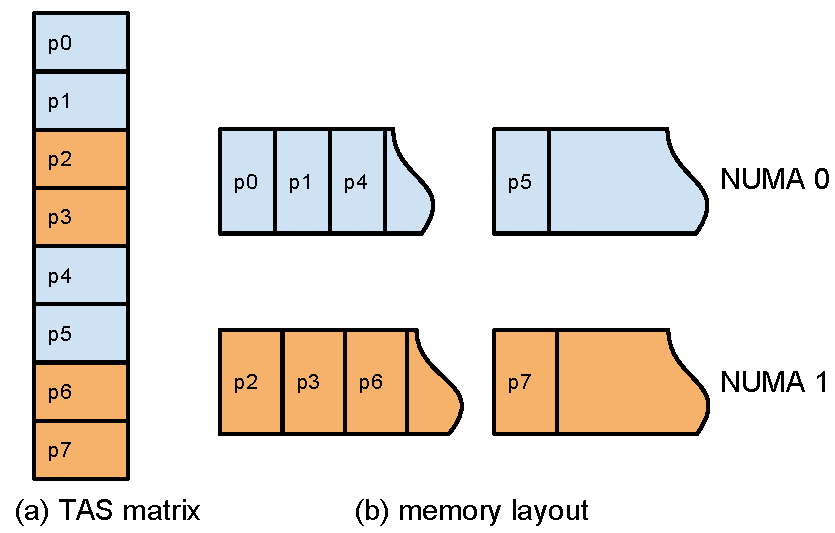
\includegraphics[scale=0.5]{./matrix_mem.pdf}
	\caption{Memory layout of a tall-and-skinny dense matrix.}
	\label{fig:mat_mem}
\end{figure}

FlashMatrix stores an in-memory matrix in fixed-size memory chunks and
recycles memory chunks to reduce memory allocation overhead (Figure
\ref{fig:mat_mem}). FlashMatrix requires only an I/O-level partition to
be stored in contiguous memory. As long as a memory chunk is sufficient
to store an I/O-level partition, FlashMatrix can store a matrix in a set
of fixed-size memory chunks. The size of a memory chunk is a global parameter
and is the same for all matrices. As such, FlashMatrix can reuse memory chunks
allocated for matrices of different shapes. In practice, the memory chunk size
may not be divisible by an I/O-level partition size. Therefore, the memory chunk
size is much larger than the I/O-level partition size to increase
memory utilization. We use 64MB as the default memory chunk size.

FlashMatrix maintains per-thread memory buffer pools to access I/O-level
partitions of a matrix on SSDs. These memory buffers have the same size as
I/O-level partitions, which is in the order of megabytes to maximize I/O
throughput of an SSD. Because all partitions of a matrix have the same size,
the memory buffers are reused.

\subsection{Implementation of GenOps with VUDF}

FlashMatrix invokes VUDFs on the elements of CPU-level partitions intelligently
to reduce the overhead of function calls. Different GenOps choose different
forms of VUDFs based on the data layout and the shape of the input matrices.

Some GenOps are applied to matrices with any data layout and any shape
efficiently. For example, \textit{sapply} and \textit{mapply} only require
the input matrices and the output matrix to have the same data layout. For tall
column-major matrices and wide row-major matrices, each CPU-level partition has
long columns and long rows, respectively. As such, these GenOps invoke a VUDF
on the long columns and rows. For tall row-major matrices and wide column-major
matrices, all rows and columns in a CPU-level partition is stored in a single
piece of memory. As such, these GenOps invoke a VUDF only once on all
elements in a partition. %A similar strategy is applicable to \textit{agg}.

Most of the GenOps require a matrix with
a specific data layout to increase the amortization of function call overhead.
Many of the GenOps favor the column-major order for a tall-and-skinny matrix
and the row-major order for a short-and-wide matrix. These data layouts increase
the length of a vector passed to a VUDF and align data in memory. For example,
the column-major order ensures that each column in a partition of a tall matrix
is well aligned in memory owing to the matrix format and the partition size
(Figure \ref{fig:tas_mat}), regardless of the number of columns in the matrix.
A GenOp
such as inner product converts the data layout of a CPU-level partition to
the preferred layout if an input matrix does not have the preferred layout.
%Because a CPU-level partition fits in the CPU cache, data layout conversion
%does not increase data access to main memory. 

Given a matrix with the preferred data layout, FlashMatrix automatically
selects the right form of a VUDF for a given GenOp. For example, when applying
\textit{mapply\_col} on a tall column-major matrix, FlashMatrix invokes
the \textit{bVUDF1} form of the binary VUDF on a column from the input matrix
and the input vector; when applying \textit{mapply\_row} on a tall column-major
matrix, FlashMatrix invokes the \textit{bVUDF2} form on a column from the input
matrix and an element from the vector. When applying \textit{inner\_prod\_tall}
on a tall column-major matrix, FlashMatrix uses the \textit{bVUDF2} form of
the first VUDF to computes the outer product of a column from the left matrix
and a row from the right matrix and uses the \textit{aVUDF2} of the second VUDF
to compute the final result. Because \textit{inner\_prod\_tall} operates on
a CPU-level partition, all intermediate results in the computation are kept
in CPU cache. \textit{inner\_prod\_wide} invokes the
\textit{bVUDF1} form of the first VUDF on a row from the left matrix and a column
from the right matrix and invokes the \textit{aVUDF1} form of the second VUDF
on the output from the first VUDF to compute an element in the output matrix for
the input partitions.

%Both \textit{agg\_row} and \textit{agg\_col} work better on the preferred data
%layout if the aggregation VUDF has the same \textit{aggregate} and \textit{combine}
%function with both \textit{aVUDF1} and \textit{aVUDF2} forms. For these aggregation
%VUDFs, we can transform \textit{agg\_row} on a column-major matrix to applying
%\textit{aVUDF2} to columns of a partition. Similar transformation is applied
%to \textit{agg\_col} on a row-major matrix.

%Inner product chooses different forms of VUDFs for input matrices with different
%shapes. The first UDF of inner product is a binary UDF and the second one is an
%aggregation UDF. For the sake of efficiency, inner product requires the second
%UDF to have the same \textit{aggregate} and \textit{combine} function with both
%\textit{aVUDF1} and \textit{aVUDF2} forms.

%Unlike other GenOps, \textit{groupby\_row} and \textit{groupby\_col} are the only
%GenOps that do not favor the column-major order for a tall-and-skinny matrix and
%the row-major order for a short-and-wide matrix. \textit{groupby\_row} sorts
%rows in a partition based on the categorical values associated with each row
%and apply the aggregation VUDF on rows directly.

\subsection{Implementation of GenOps on a group of matrices} \label{sec:group_op}

When applying a GenOp on a group of matrices (Section \ref{sec:mat_group}),
we decompose the computation into multiple GenOps and apply them to individual
matrices in the group if the GenOp supports decomposition. Decomposing computation
to individual matrices reduces memory copy and increases CPU cache hits.
For the GenOps that cannot be decomposed, we combine the individual matrices
on the fly and apply the GenOps on the combined matrix directly.

We apply some of the GenOps to individual matrices directly without
transformation. For example,
\textit{sapply} and \textit{agg} run on individual matrices directly regardless
of the shape and data layout of the matrices. Other GenOps may be applied
to individual matrices directly if the input matrices have certain shape. For
example, we apply \textit{mapply\_col} and \textit{agg\_col} to individual
matrices in a group of tall matrices directly.  Similarly, we apply
\textit{mapply\_row} and \textit{agg\_row} to
individual matrices in a group of wide matrices directly. %\textit{mapply}
%requires the matrices in the two input matrix groups to have the same shape.
%\textit{Groupby\_row} on a \textit{tall matrix group} can be decomposed and
%applied to individual matrices; \textit{groupby\_col} on a \textit{wide matrix group}
%can be decomposed in a similar fashion.

Applying other GenOps to a group of matrices requires transformation. If an aggregation
VUDF provides a \textit{combine} function, applying \textit{agg\_row} to a group of
tall matrices is transformed into two steps: apply the \textit{aggregate} function on
each row of individual matrices and apply the \textit{combine} function on the partial
aggregation results. When applying \textit{mapply\_row} to a group of tall matrices,
we break the input vector into parts to match the number of columns in the individual
matrices in the group and apply \textit{mapply\_row} to individual matrices
separately. The same strategies are used for \textit{agg\_col} and
\textit{mapply\_col} on a group of wide matrices. 

%FlashMatrix decomposes inner product on a matrix group in favor of minimizing
%the amount of data written to SSDs (Figure \ref{fig:inner_prod}).
%For \textit{inner\_prod\_tall}, we first partition the right matrix vertically
%so that the inner product of the left matrix and a vertical partition outputs
%part of a final output matrix. The number of vertical partitions determines
%the number of runs required to complete the inner product on the group of matrices.
%If the left matrix is stored on SSDs, the number of vertical partitions on
%the right matrix determines the amount of data read from SSDs. The vertical
%partition size determines the output matrix size in each run and affect
%the memory size. As such, we need to select the vertical partition size of
%the right matrix to balance I/O and memory consumption. We horizontally partition
%each vertical partition of the right matrix to further decompose the inner
%product. We construct a directed acyclic graph (DAG) to evalute the inner
%product lazily (Section \ref{sec:lazy_eval}). Similarly, we partition the right
%matrix and make a similar choice to balance I/O and memory consumption for
%\textit{inner\_prod\_wide}. We also construct a DAG and lazily evaluate
%the computation.

%\begin{figure}
%\centering
%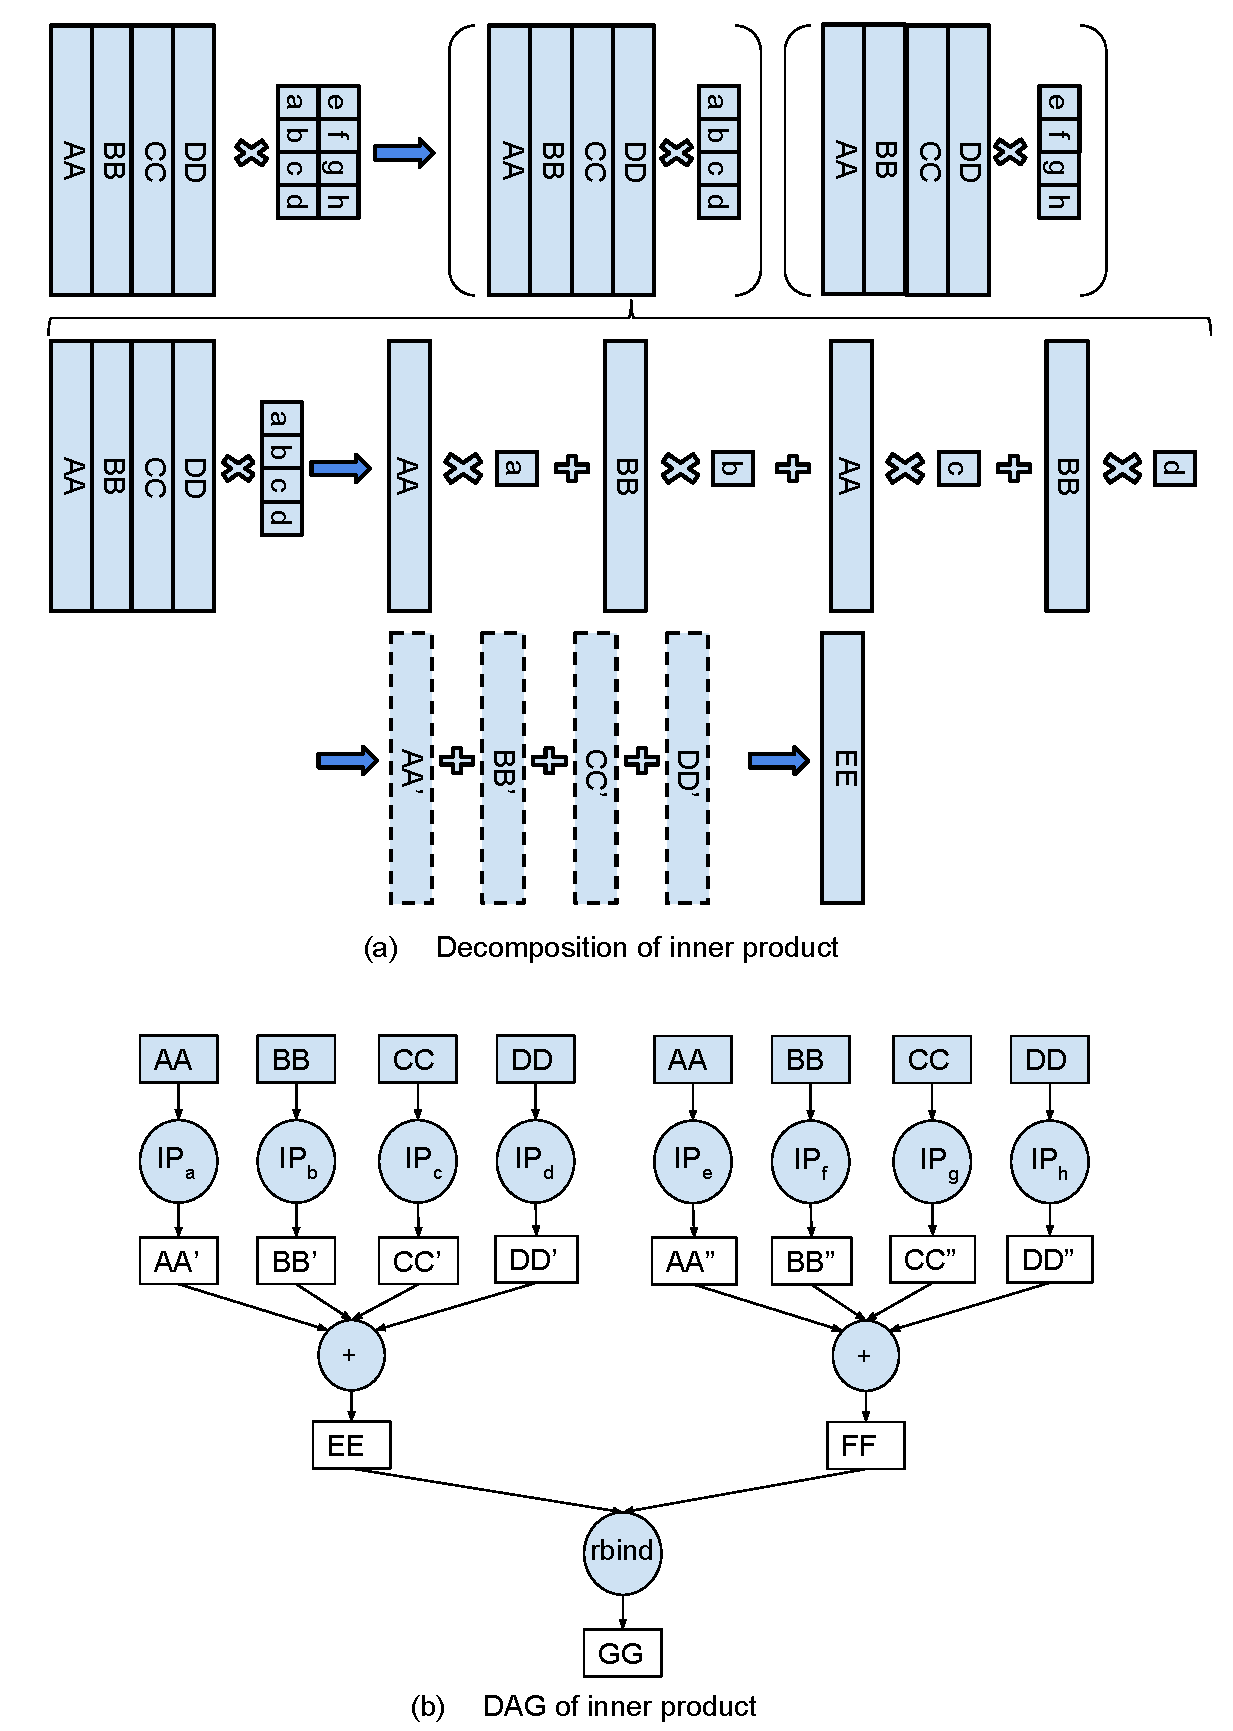
\includegraphics[scale=0.4]{./inner_prod_tall.pdf}
%\vspace{-5pt}
%\caption{Decomposition inner product on a group of dense matrix.}
%\vspace{-5pt}
%\label{fig:inner_prod}
%\end{figure}
